\section{Experiments}

\begin{frame}{Experiments}
    \begin{itemize}
        \item Different parameter settings for each hypothesis
        \item Each experiment is run 100 times
        \item Experiment end statistics are written to files
        \item Test method: two-sample t-test % to determine whether the difference between means found in the sample is significantly different from the hypothesized difference between two means
        \item Significance level: 0.05
        \item Hypotheses entail one-tailed tests. Null hypothesis will be rejected if the mean difference between sample means is too small.

        %\pause
        \item[]
        \item Could not experiment with varying dynamism because of an error with RinSim Experiment repeats we couldn't fix
    \end{itemize}
\end{frame}


\begin{frame}{Experiments: Question 1 (1)}
    \begin{itemize}
        \item What is the relation between the amount of requests that RoboPizza receives and the waiting time for customers?
        \begin{itemize}
                \item $H_1$: The waiting time increases with the amount of requests.
                \item $H_0$: The waiting time does \textbf{not} increase with the amount of requests.
        \end{itemize}

        \item[]
        \item TODO: Hypotheses in termen van $H_0: \mu_1 \geq \mu_2$ en $H_1: \mu_1 < \mu_2$
        \item http://stattrek.com/hypothesis-test/difference-in-means.aspx
    \end{itemize}
\end{frame}


\begin{frame}{Experiments: Question 1 (2)}
    \begin{itemize}
        \item Total task waiting time
    \end{itemize}

    \begin{figure}[hbt]
        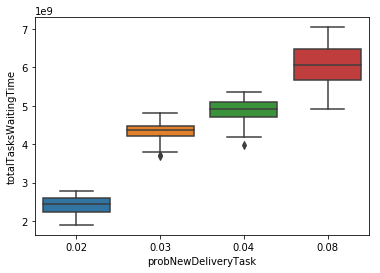
\includegraphics[width=8cm]{imgs/question1-plot1}
    \end{figure}
\end{frame}


\begin{frame}{Experiments: Question 2 (1)}
    \begin{itemize}
        \item Do robots drive more (non-idle time) when there are more requests in the system?
        \begin{itemize}
                \item $H_1$: Robots drive more when there are more requests in the system.
                \item $H_0$: Robots do \textbf{not} driving more when there are more requests in the system.
        \end{itemize}

        \item[]
        \item TODO: Hypotheses in termen van $H_0: \mu_1 \geq \mu_2$ en $H_1: \mu_1 < \mu_2$
        \item http://stattrek.com/hypothesis-test/difference-in-means.aspx
    \end{itemize}
\end{frame}

\begin{frame}{Experiments: Question 2 (3)}
    \begin{itemize}
        \item Total tasks
    \end{itemize}

    \begin{figure}[!hbt]
        \centering
        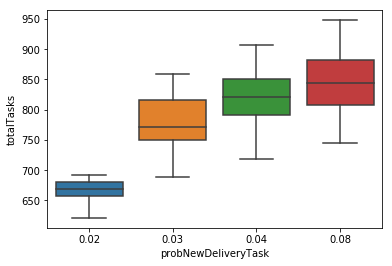
\includegraphics[width=8.5cm]{imgs/question2-plot3}
    \end{figure}
\end{frame}

\begin{frame}{Experiments: Question 2 (2)}
    \begin{itemize}
        \item Total idle and travel time
    \end{itemize}

    \begin{figure}[!hbt]
        \begin{adjustbox}{center}
            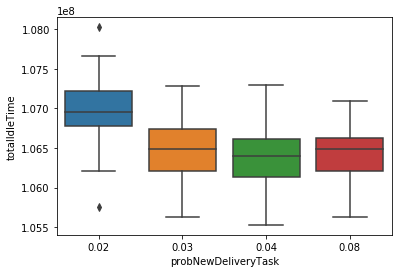
\includegraphics[width=6cm]{imgs/question2-plot1}
            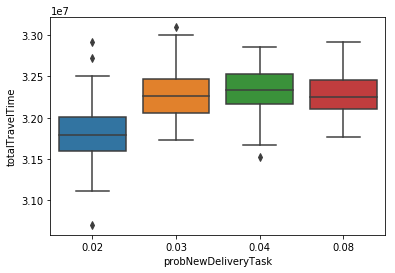
\includegraphics[width=6cm]{imgs/question2-plot2}
        \end{adjustbox}
    \end{figure}
\end{frame}


\begin{frame}{Experiments: Question 3 (1)}
    \begin{itemize}
        \item Does increasing the amount of robots decrease customer waiting time when there are many requests?
        \begin{itemize}
                \item $H_1$: Increasing the amount of robots decreases customer waiting time when there are many requests.
                \item $H_0$: Increasing the amount of robots does \textbf{not} decrease customer waiting time when there are many requests.
        \end{itemize}

        \item[]
        \item TODO: Hypotheses in termen van $H_0: \mu_1 \geq \mu_2$ en $H_1: \mu_1 < \mu_2$
        \item http://stattrek.com/hypothesis-test/difference-in-means.aspx
    \end{itemize}
\end{frame}



\begin{frame}{Experiments: Question 3 (2)}
    \begin{itemize}
        \item grafieken ofzo
    \end{itemize}
\end{frame}

